\documentclass[12pt]{article}
\usepackage{amsmath}
\usepackage{amssymb}
\usepackage{fancyhdr}
\usepackage{geometry}
\usepackage{hanging}
\usepackage{enumitem}
\usepackage{graphicx}
\usepackage{setspace}
\usepackage{tabularx}
\usepackage{array}
\usepackage{xcolor}
\usepackage[dvipsnames]{xcolor}
\usepackage{longtable}
%\usepackage{lipsum} %remove later
\doublespacing
%\setlength\parindent{28 pt}
\geometry{letterpaper, margin=1in}

% ++++ Fancy Settings (for header) ++++
\pagestyle{plain}
\fancypagestyle{main}{
	\fancyhf{}
	\lhead{Lab 09}
	\rhead{\leftmark}
	\cfoot{\thepage}
	\renewcommand{\headrulewidth}{0.4pt}
}

% Column widths (tweak the numbers if you want)
\newcommand{\colNum}{0.06\linewidth}   % column 1 (1–10)
\newcommand{\colSmall}{0.16\linewidth} % columns 2,3,5
\newcommand{\colBig}{0.48\linewidth}   % column 4 (3x colSmall)

% ++++ Begin Doc ++++

\begin{document}

% ++++ Cover Page ++++

\begin{titlepage}
\centering
\vfill

% ++Logo
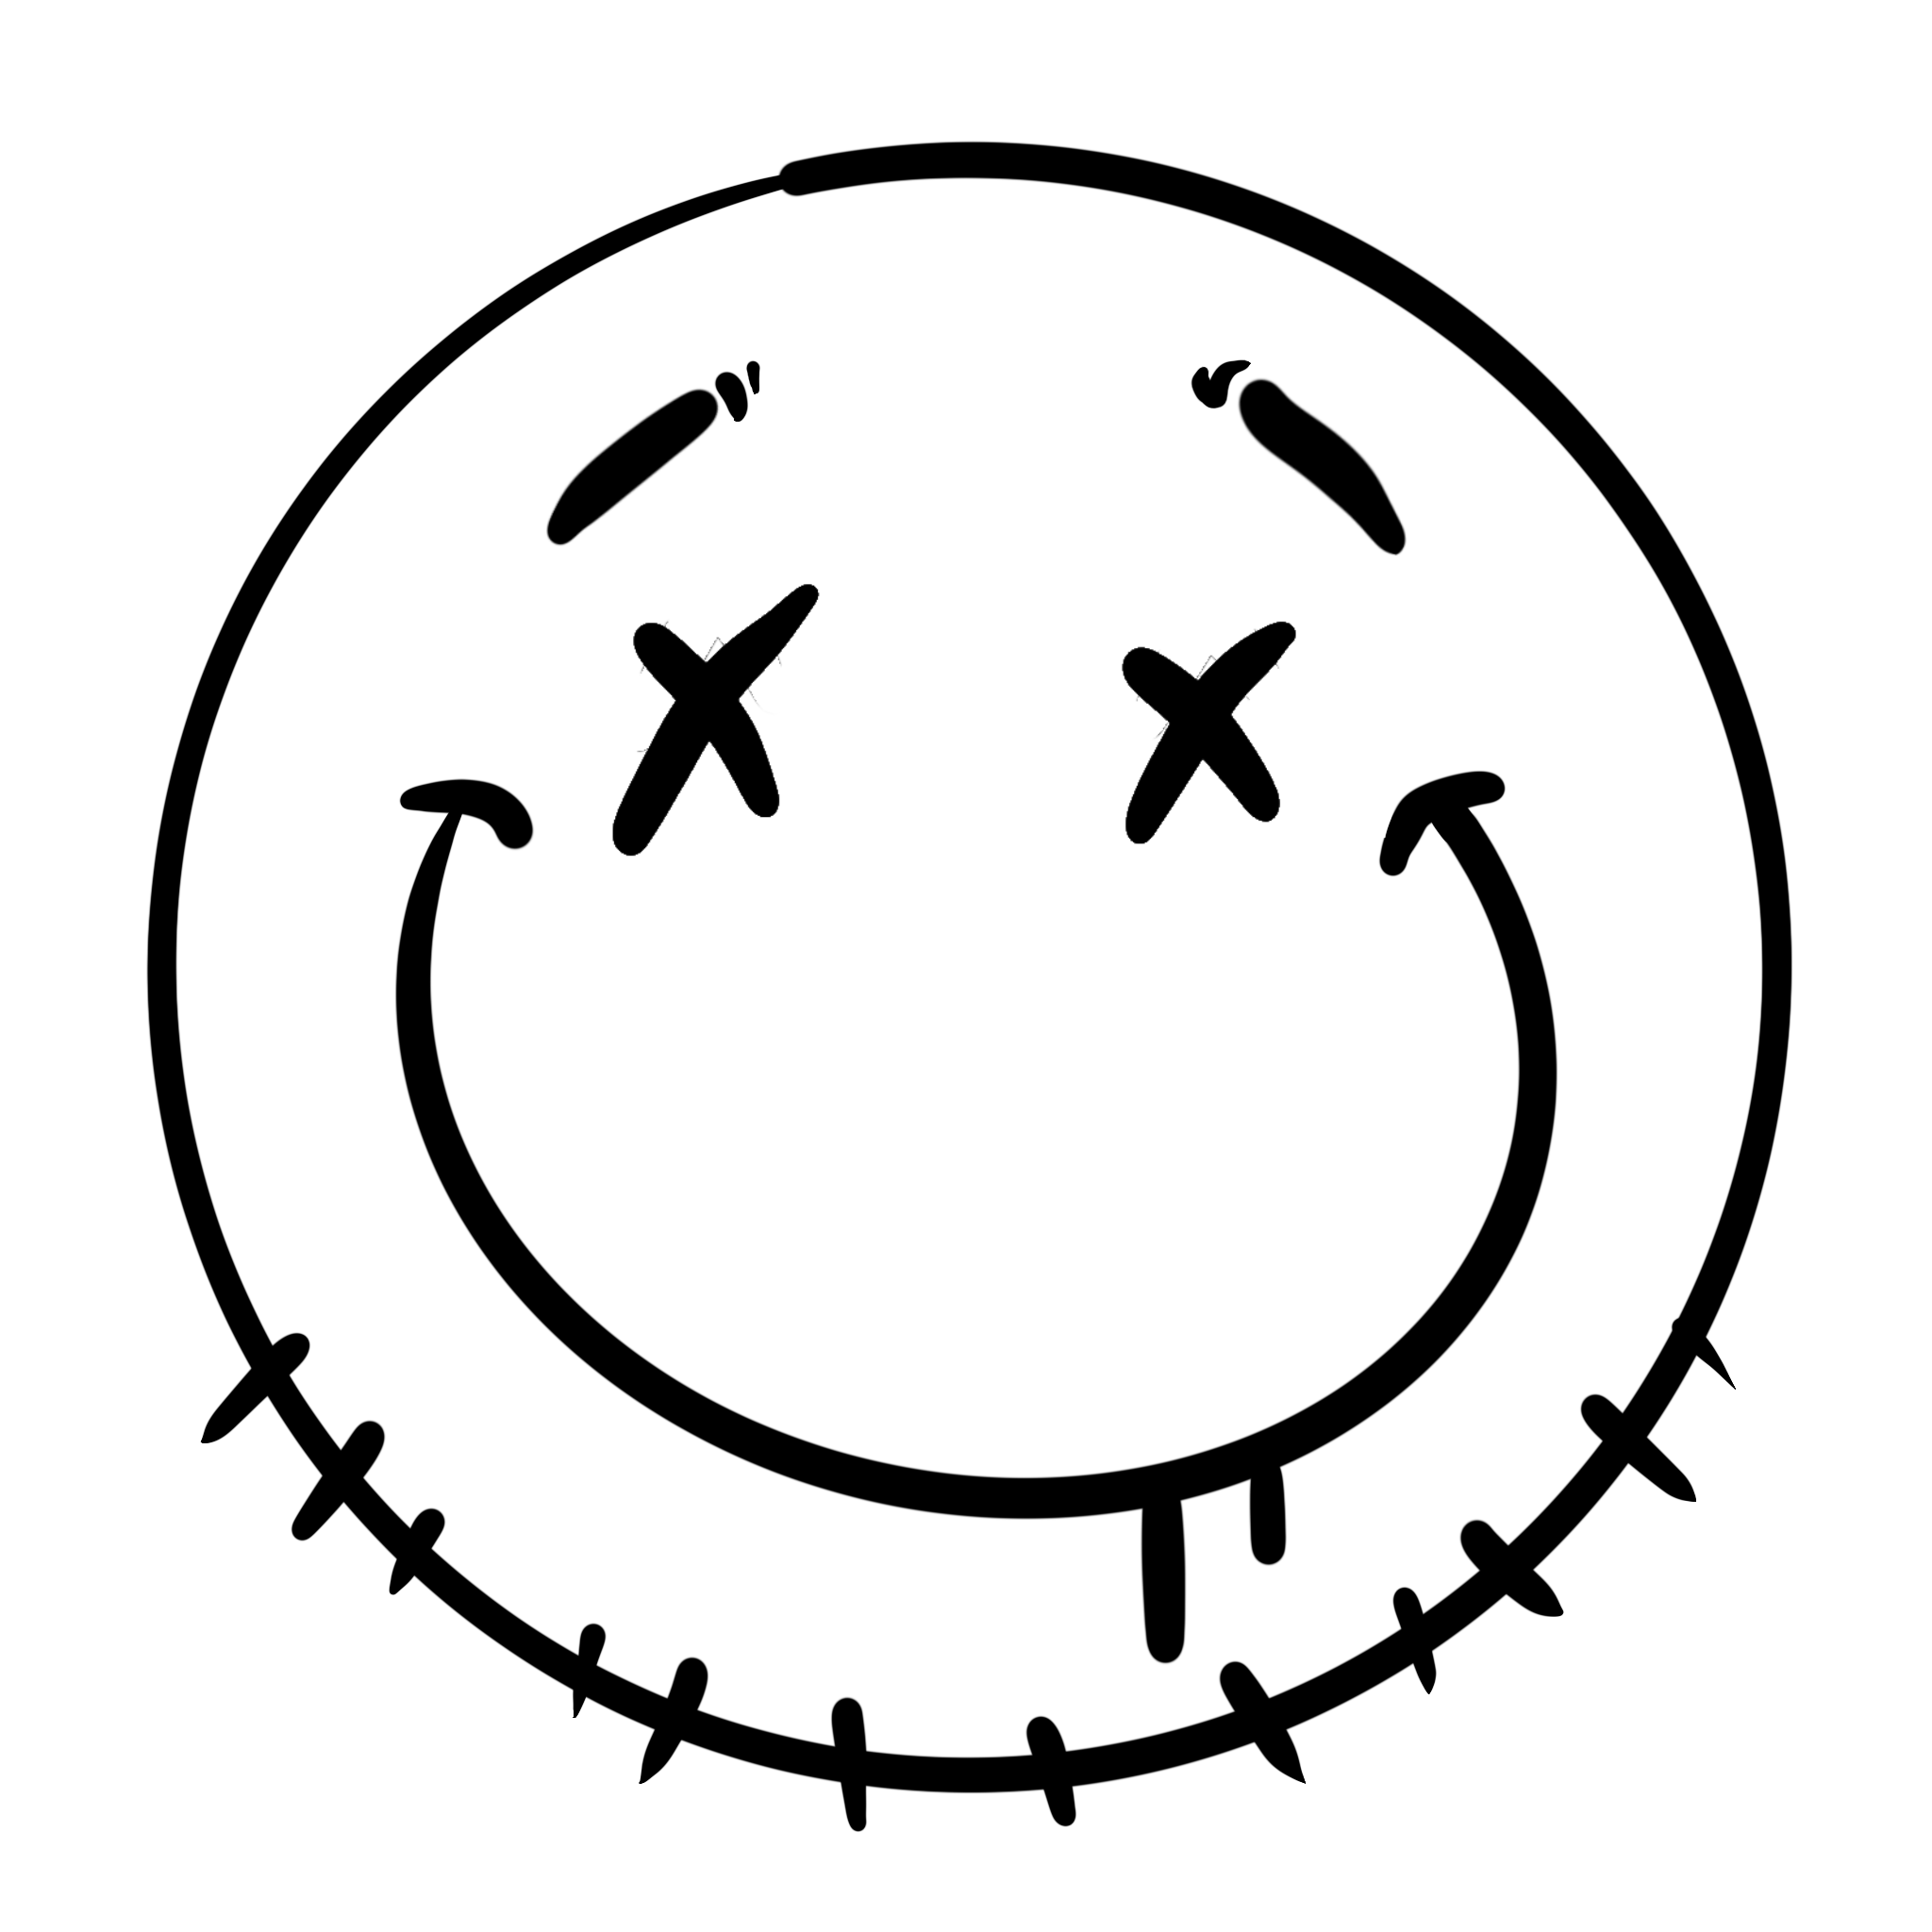
\includegraphics[width=0.35\textwidth]{images/logo.png}

\vspace{1.5cm}

% ++Title
\LARGE{\textbf{Lab 09: OS Hardening}}\\
\vspace{0.3cm}
\large{\textbf{Keith Schoen}}\\
\vspace{0.3cm}
\large{\textbf{CSEC3755-001}}\\
\vspace{0.3cm}
\large{\textbf{Dr. Daniel Pittman}}\\
\vspace{0.3cm}
\large{\textbf{8 April, 2026}}\\
\vspace{0.3cm}

\vfill
\end{titlepage}

% ++++ ToC ++++

\pagenumbering{gobble} %hide page numbers for cover and ToC
\tableofcontents
\clearpage

% ++++ Begin Report ++++

\pagenumbering{arabic} %page one starts here
\setcounter{page}{1}
\pagestyle{main} %turn on fancy

% +++++ Part 01 +++++
\section{Windows Hardening}
% +++ P01.1 +++
\subsection{Review User Accounts}
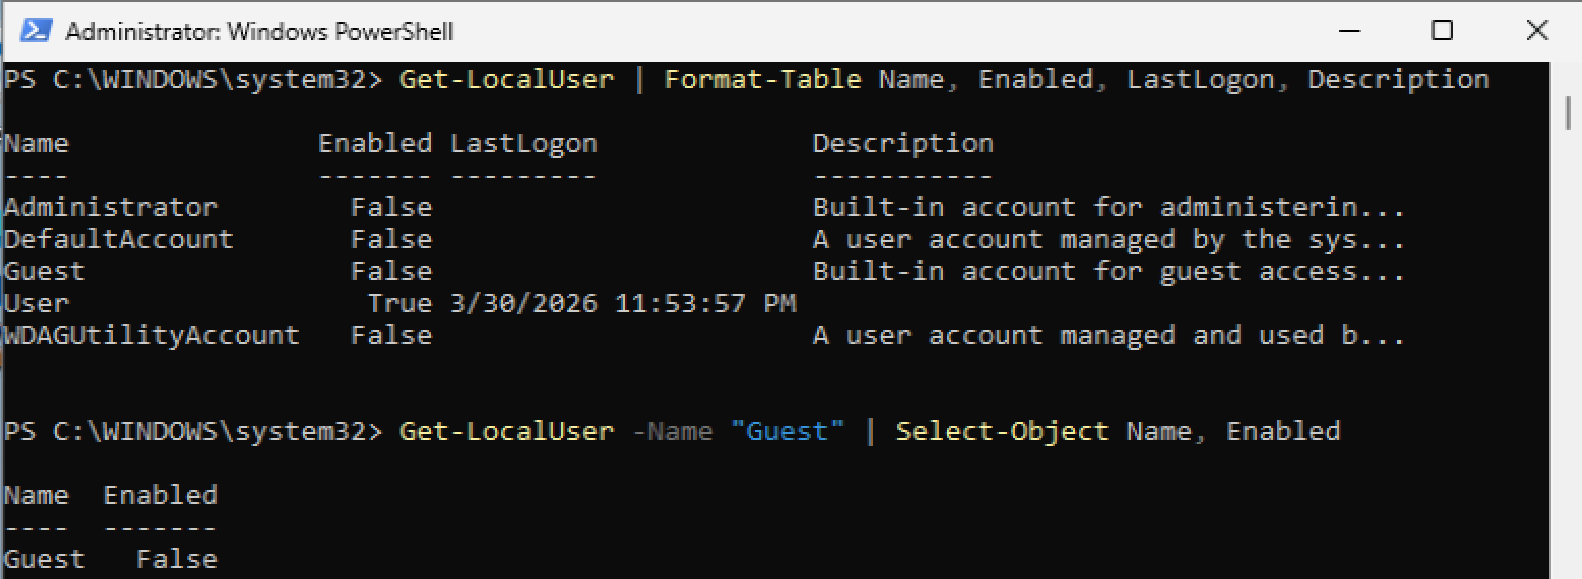
\includegraphics[width=0.50\textwidth]{images/p1.1.png}\\ \textit{Figure 1: Screenshot showing all accounts and there enabled/disabled status.}\\
From a hardening perspective, the guest account would count as an unnecessary access point. The guest account allows - although limited - access to a machine/network without any credentials eliminating the "hard part" for an attacker. This account is almost always unnecessary and should be disabled.

% +++ P01.2 +++
\subsection{Configure Password Policy}
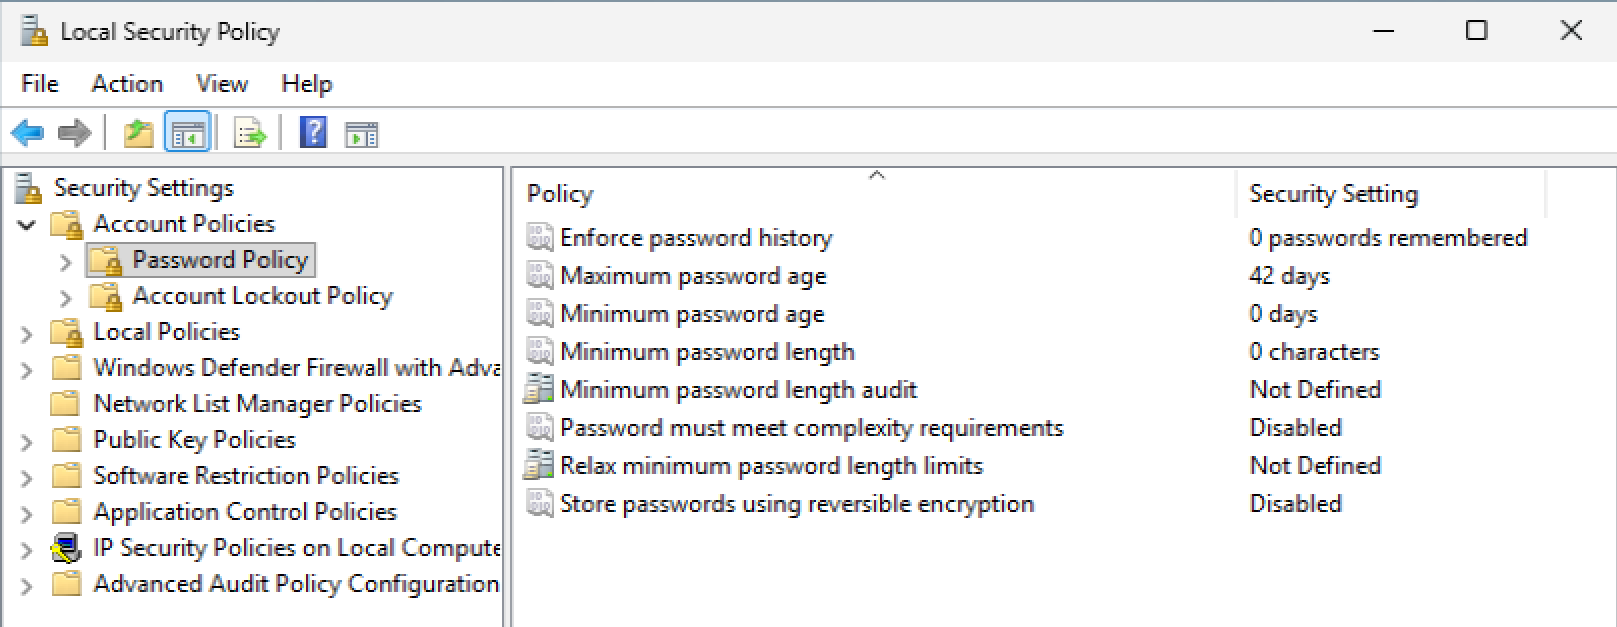
\includegraphics[width=0.50\textwidth]{images/p1.2.1.png}\\ \textit{Figure 2: Screenshot showing default password policy}\\
\ \\
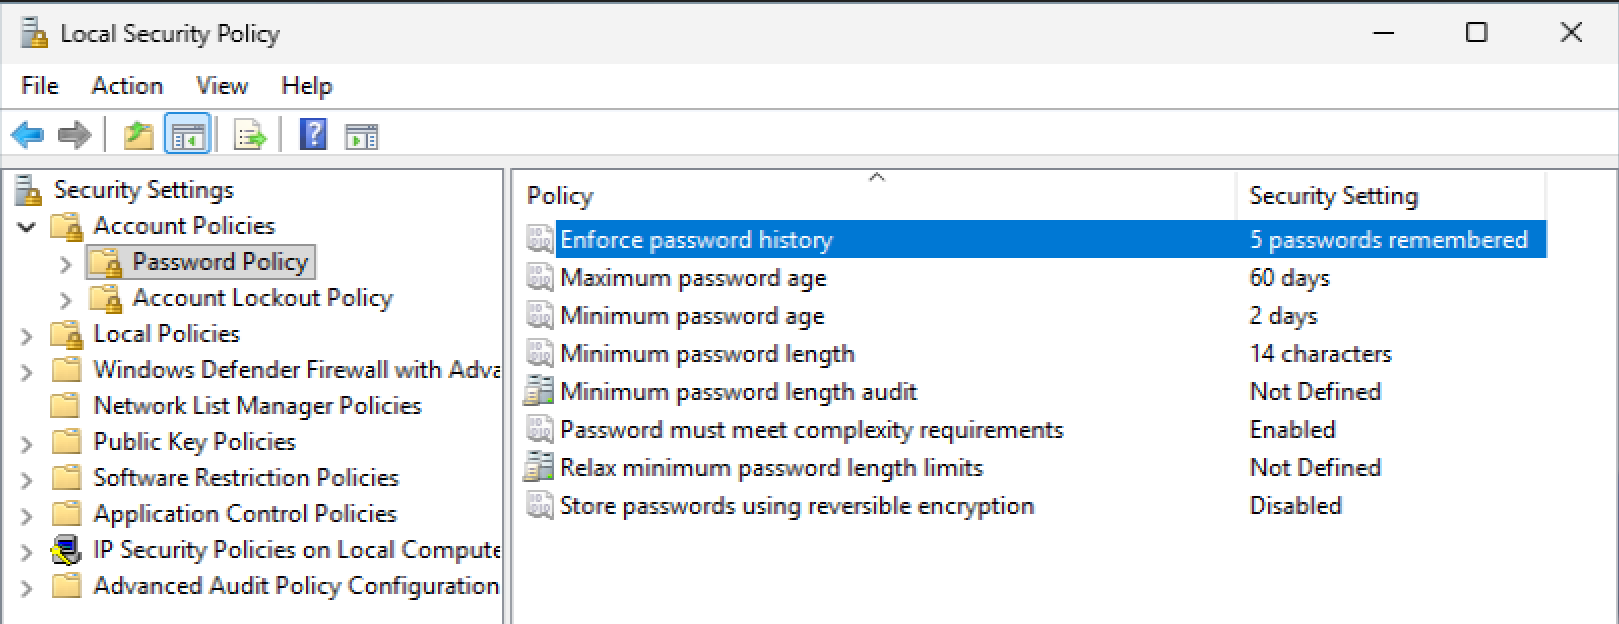
\includegraphics[width=0.50\textwidth]{images/p1.2.2.png}\\ \textit{Figure 3: Screenshot showing updated password policy}\\
People seem to hate comming up with and remembering passwords. Without having password minimums in place, everyone's password would be "user" and every machine and system would be better off without password protection (at least people would be able to get on quicker!) To make sure that password protection is doing it's bare minimum, these simple policies must be put into place.

% +++ P01.3 +++
\subsection{Configure Account Lockout Policy}
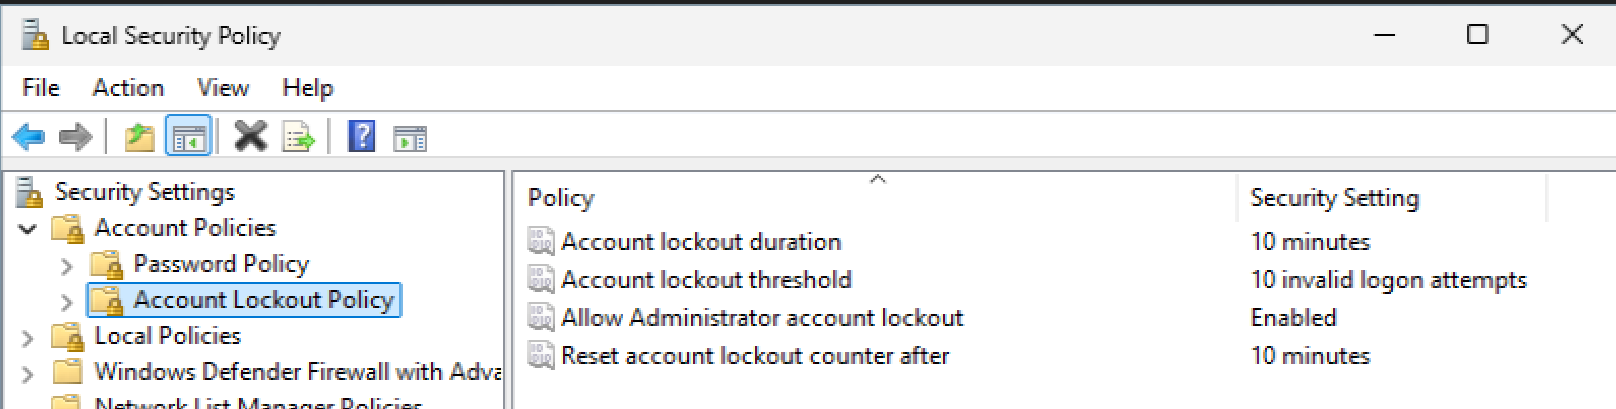
\includegraphics[width=0.50\textwidth]{images/p1.3.1.png}\\ \textit{Figure 4: Screenshot showing default lockout policy}\\
\ \\
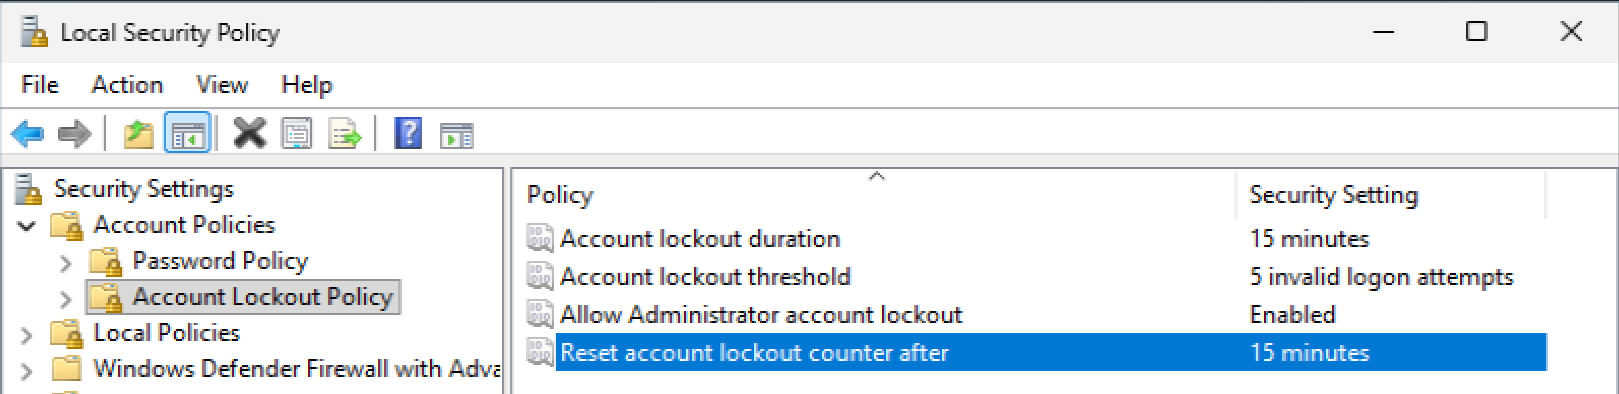
\includegraphics[width=0.50\textwidth]{images/p1.3.2.png}\\ \textit{Figure 5: Screenshot showing updated lockout policy}\\
It's not wise to give people too many tries or too much time with logging into an account. Adding just a little extra strictness to these policies makes it just that much more of a pain for even brute force tactics, hopefully making it not worth while.
\newpage

% +++ P01.4 +++
\subsection{Disable Unnecessary Services}
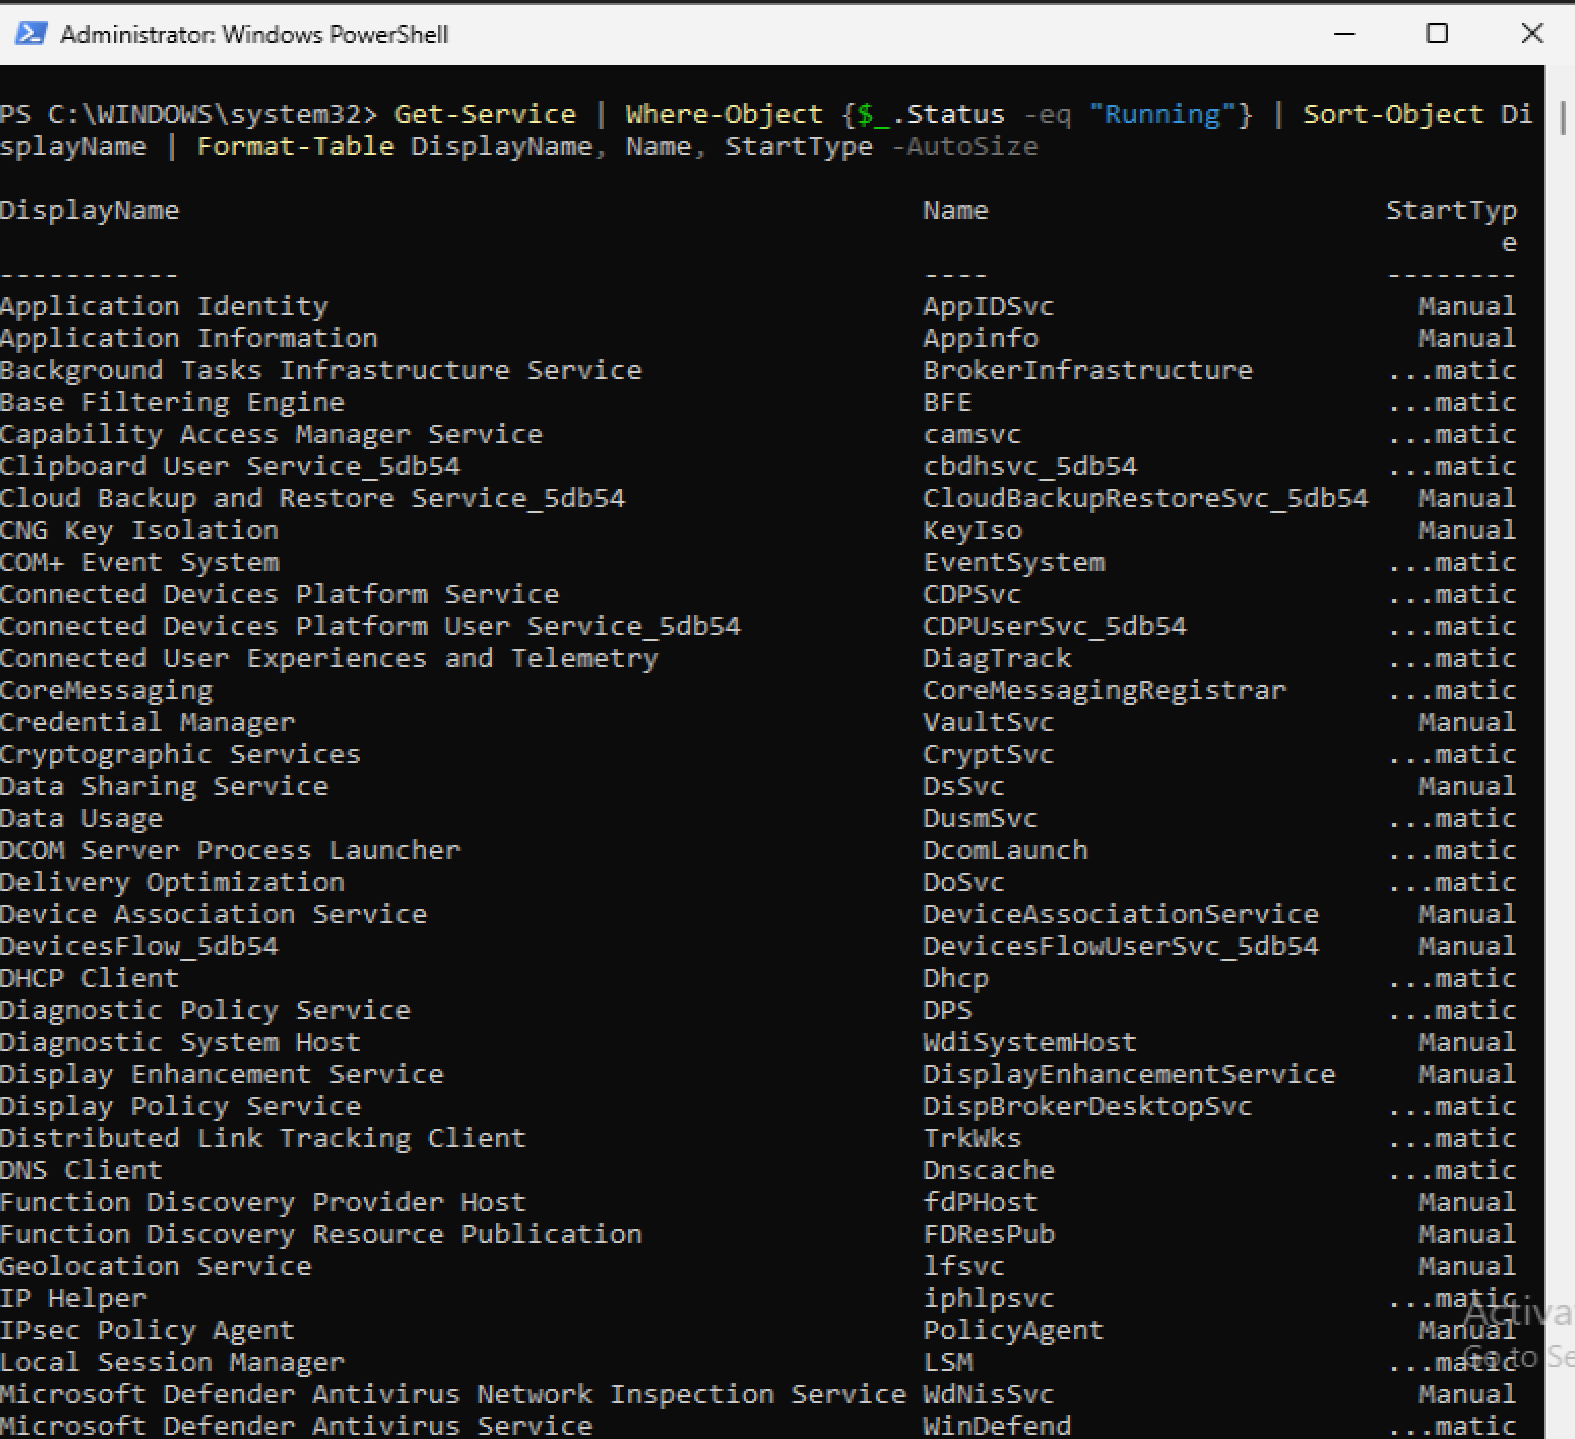
\includegraphics[width=0.32\textwidth]{images/p1.4.1.png} 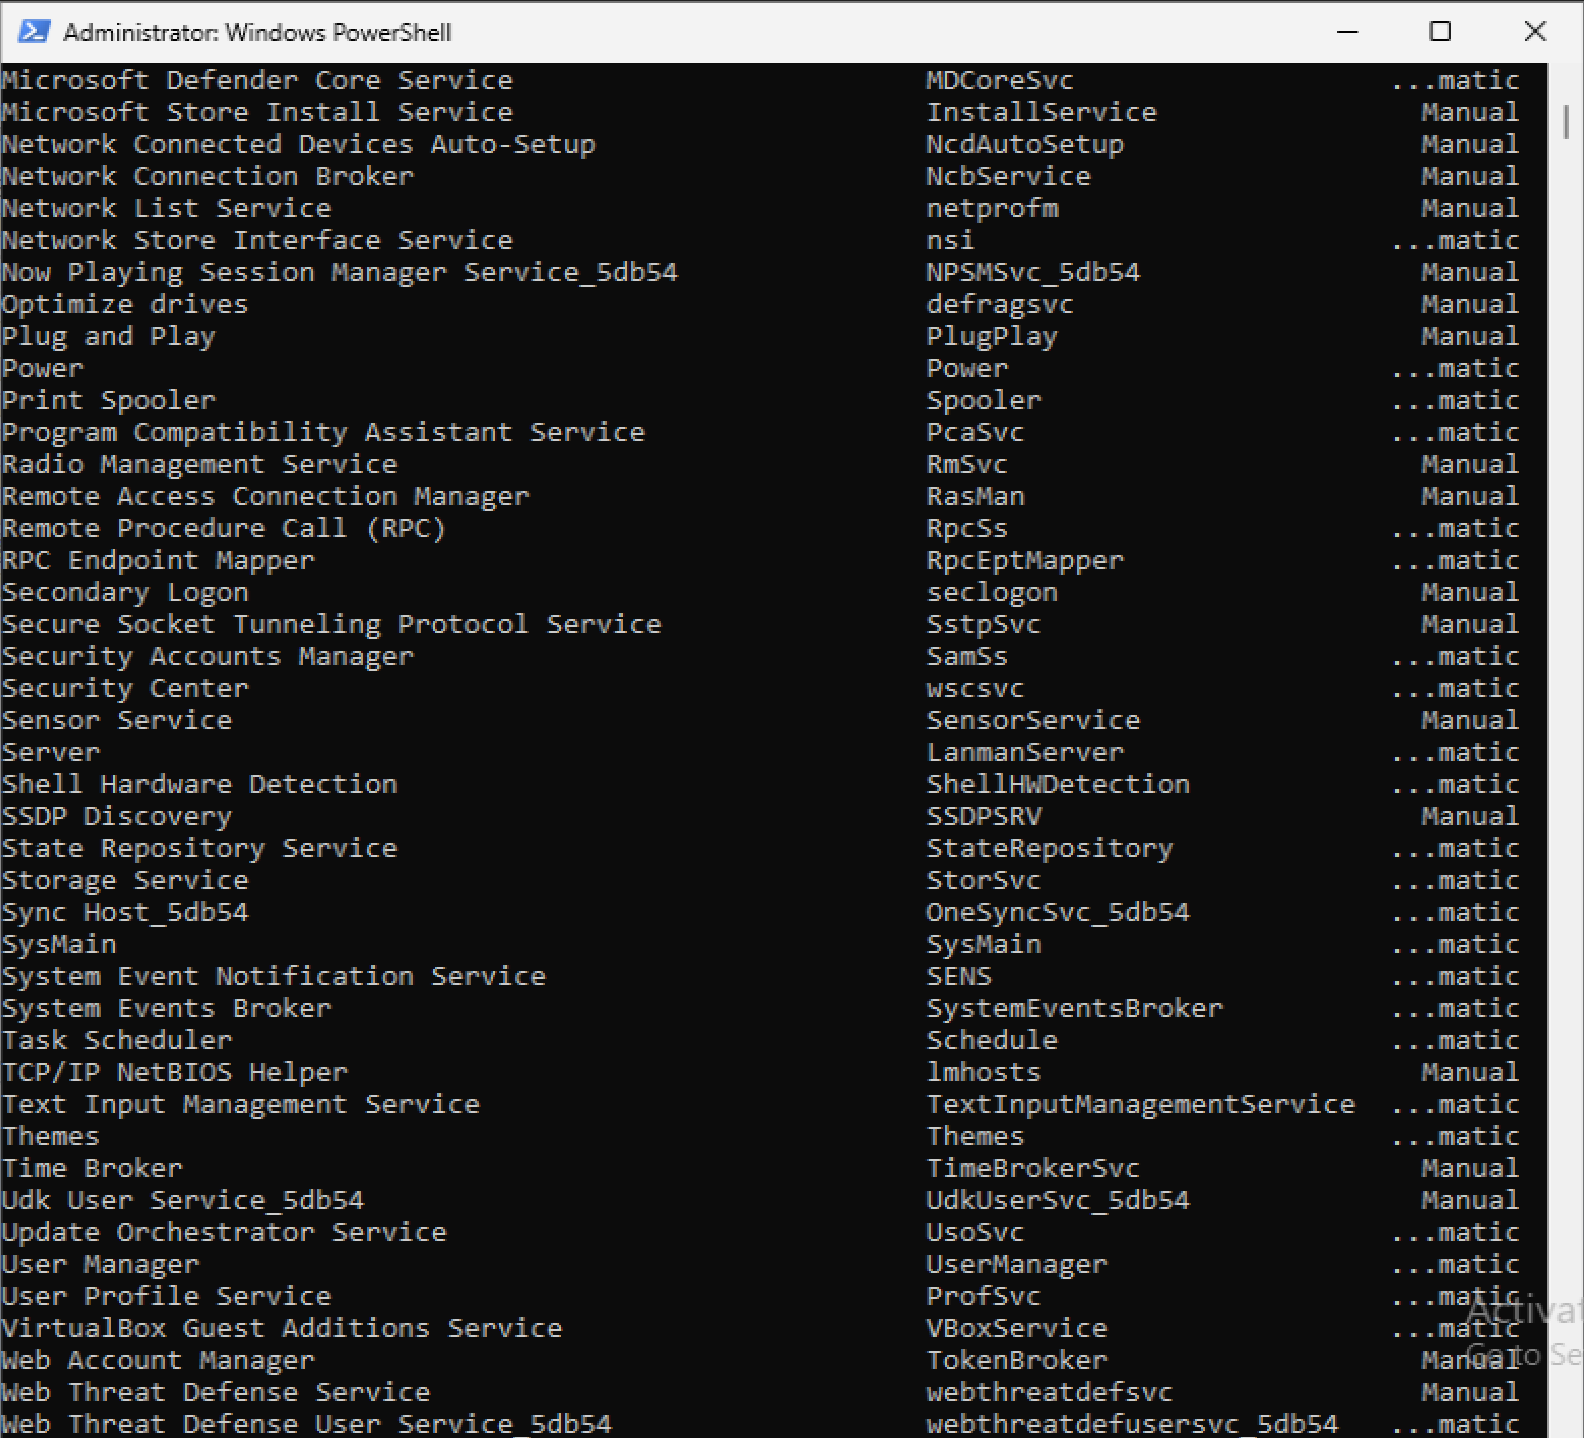
\includegraphics[width=0.32\textwidth]{images/p1.4.2.png} 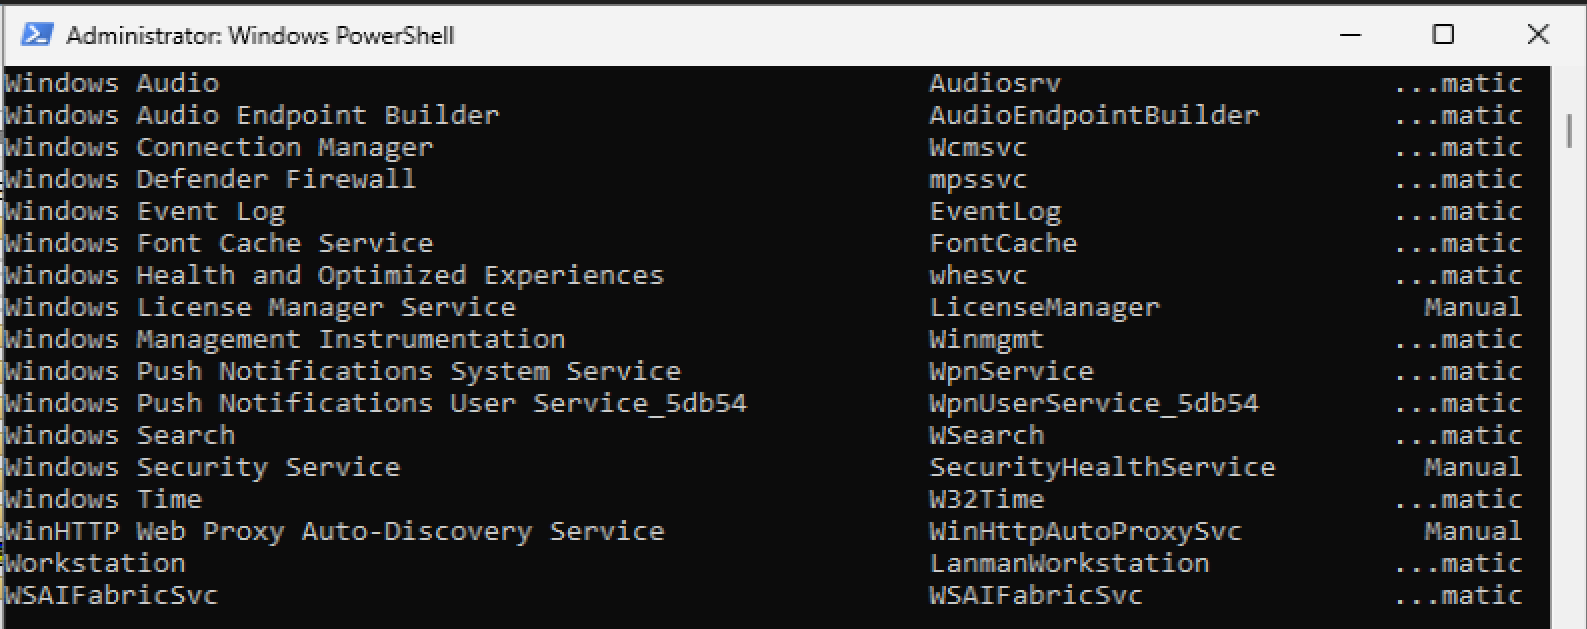
\includegraphics[width=0.32\textwidth]{images/p1.4.3.png}\\ \textit{Figures 6-8: Screenshots of the list of Running Services.}
\ \\
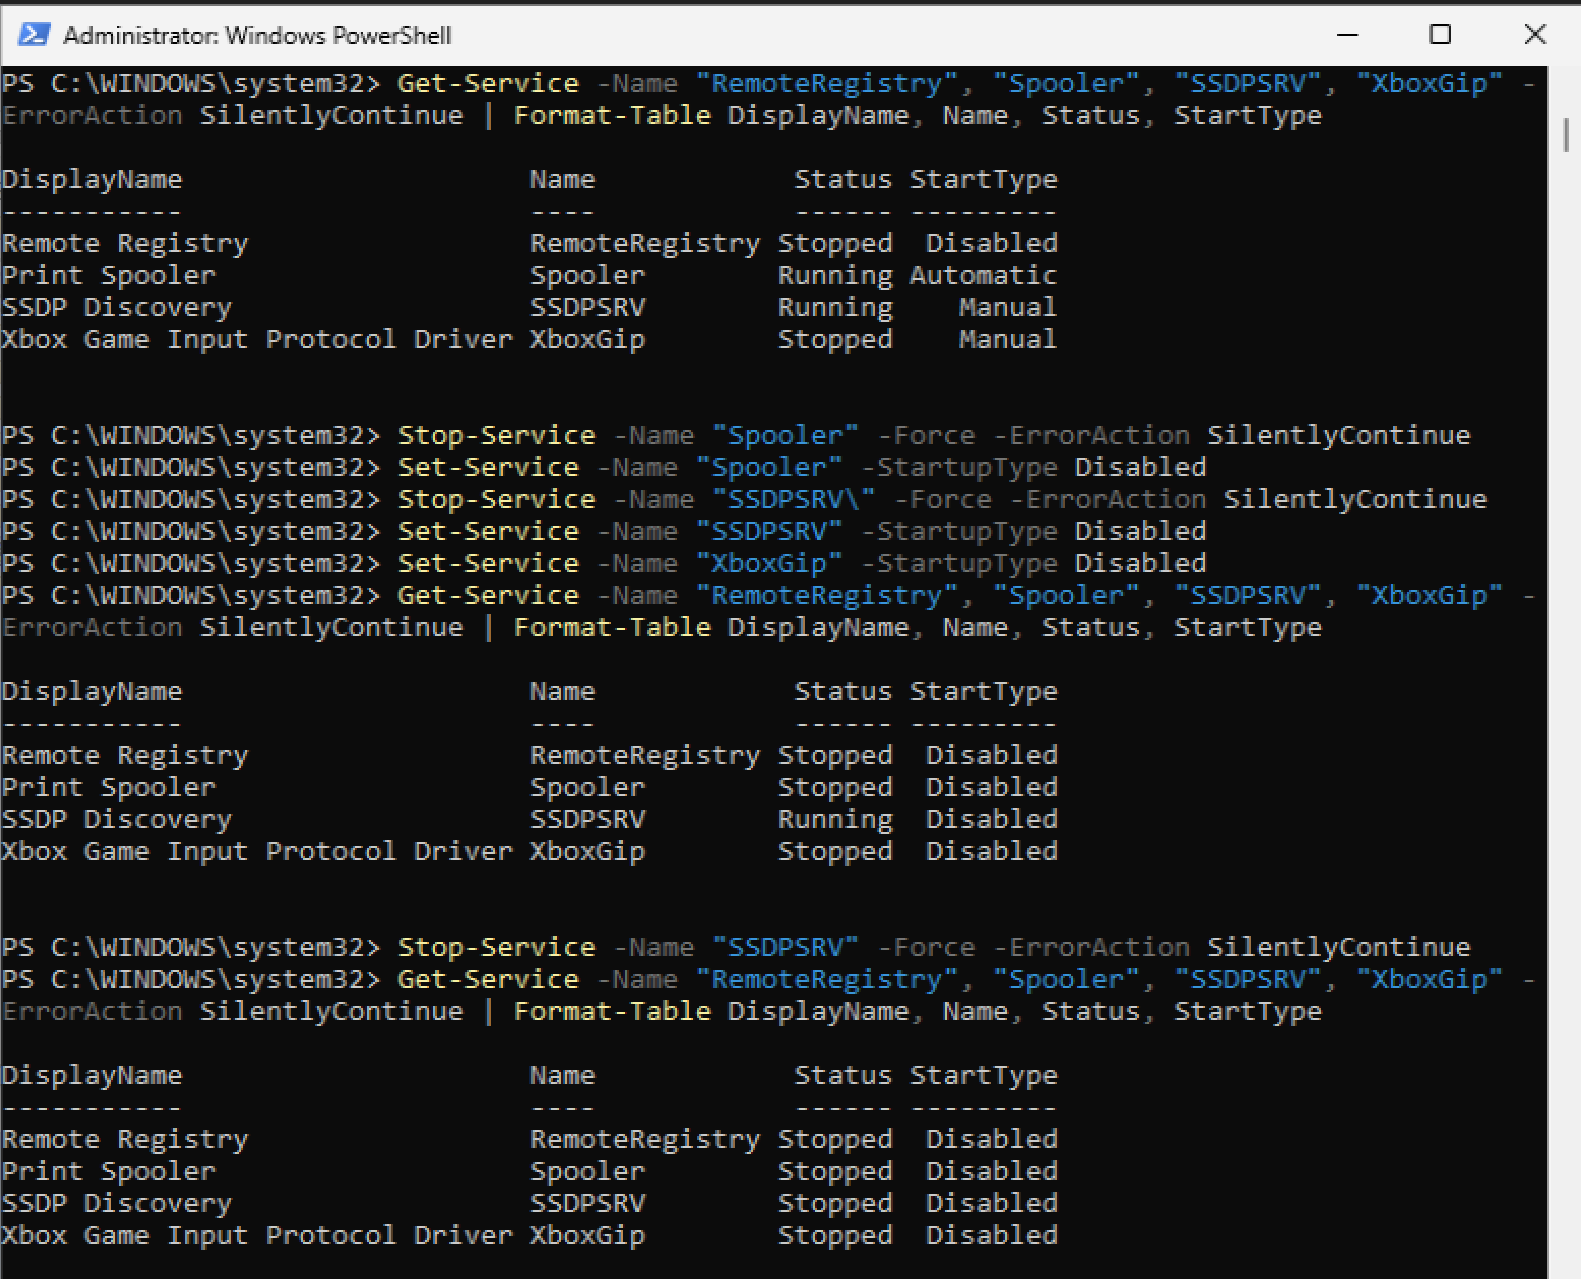
\includegraphics[width=0.50\textwidth]{images/p1.4.4.png}\\ \textit{Figure 9: Screenshot of disabled services}\\
I focused on the the 4 services that were stated as unnecessary for the VM. After running a check, I disabled the 3 that were running/enabled and stopped/disabled them.
\newpage

% ====================================================
% +++++ Part 02 +++++
\section{Linux Hardening}
% +++ P02.1 +++
\subsection{Review User Accounts in /etc/passwd}
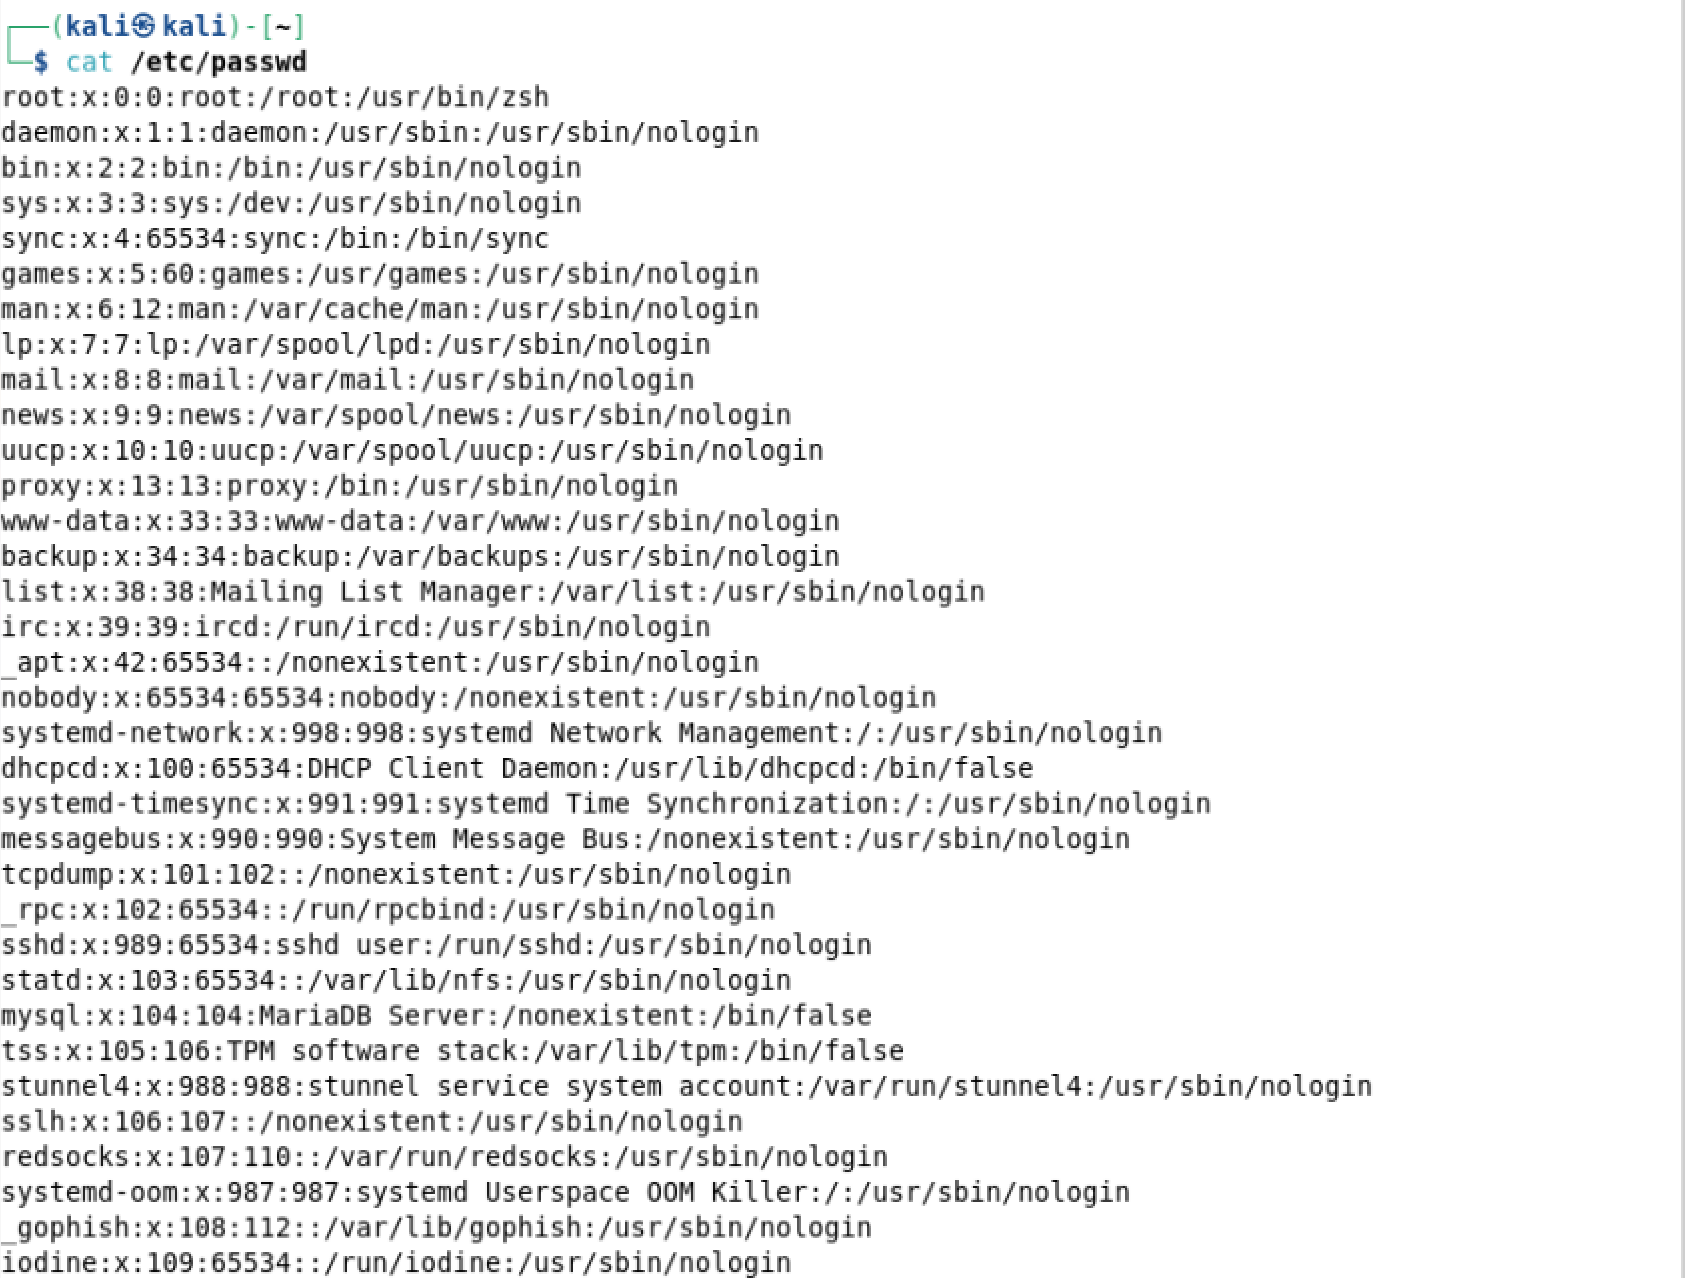
\includegraphics[width=0.46\textwidth]{images/p2.1.1.png} 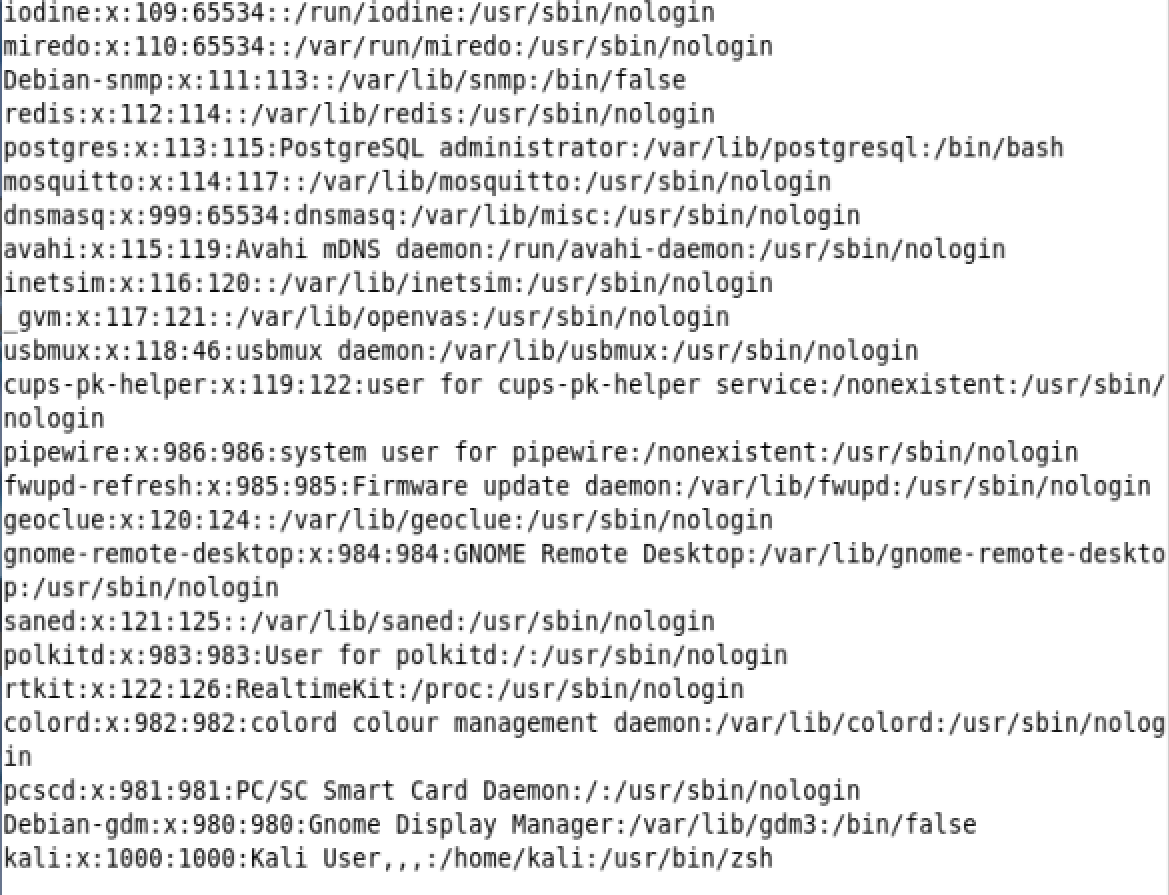
\includegraphics[width=0.46\textwidth]{images/p2.1.2.png}\\ \textit{Figures 10-11: Screenshots of all accounts}\\
\ \\
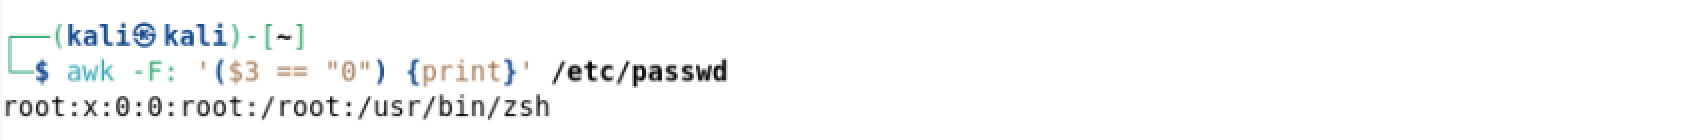
\includegraphics[width=0.50\textwidth]{images/p2.1.3.png}\\ \textit{Figure 12: Screenshot of accounts with UID 0}\\
\ \\
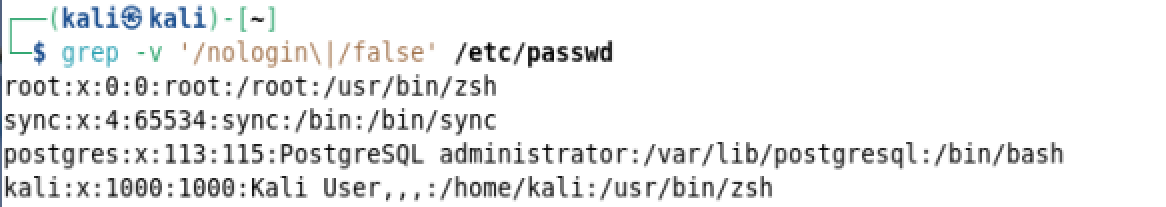
\includegraphics[width=0.50\textwidth]{images/p2.1.4.png}\\ \textit{Figure 13: Screenshot of accounts that can log in}\\
Besides the root user, there are a couple of additional accounts like kali and postgres. Based on pased labs, I think these both have something to do with the VM storage architecture.

% +++ P02.2 +++
\subsection{Configure Password Policy via /etc/login.defs}
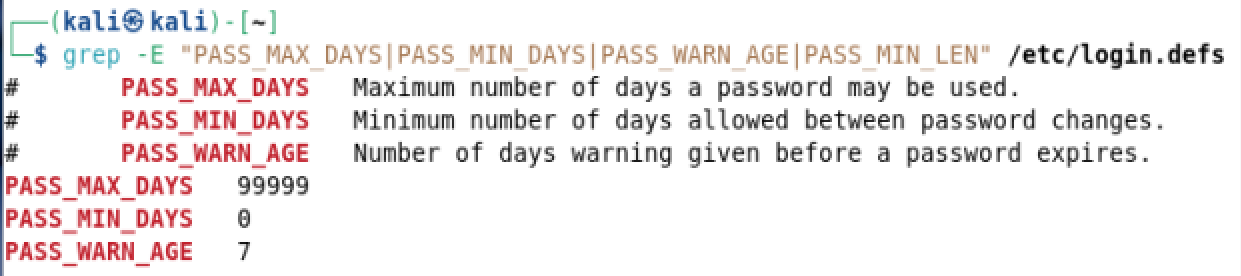
\includegraphics[width=0.50\textwidth]{images/p2.2.1.png}\\ \textit{Figure 14: Screenshot of default password policies}\\
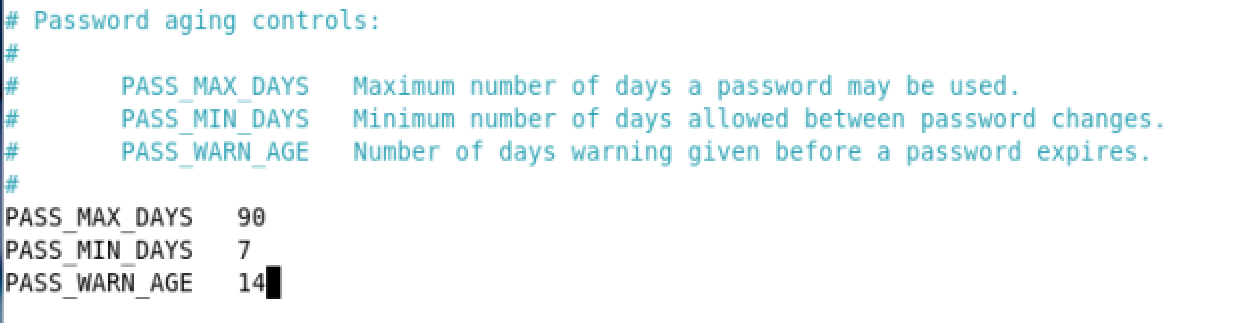
\includegraphics[width=0.50\textwidth]{images/p2.2.2.png}\\ \textit{Figure 15: Screenshot of changes to password policy in /etc/login.defs}\\
\ \\
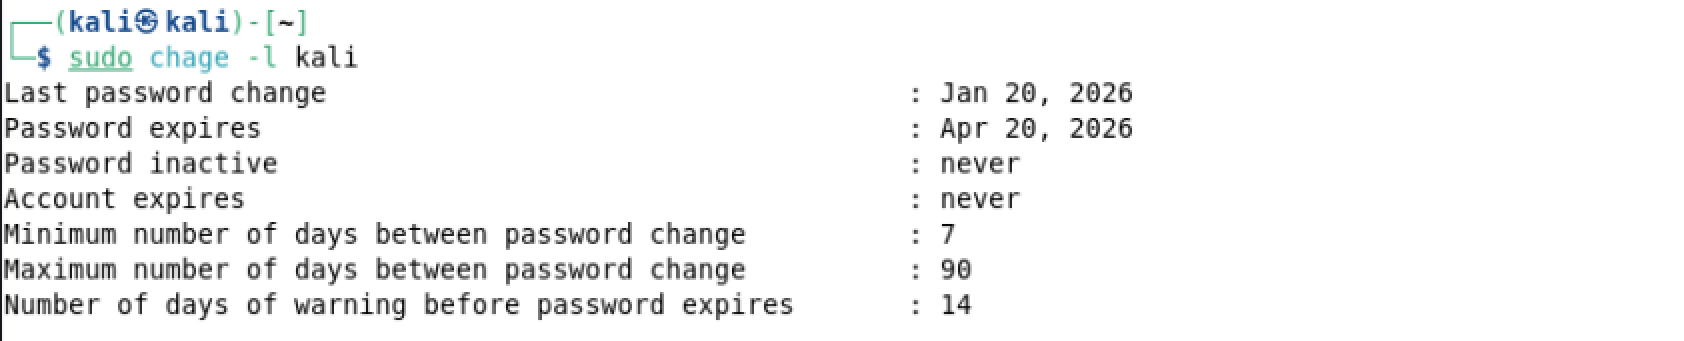
\includegraphics[width=0.50\textwidth]{images/p2.2.3.png}\\ \textit{Figure 16: Screenshot of changes to existing user kali's password policy}

% +++ P02.3 +++
\subsection{Configure Account Lockout Policy via PAM}
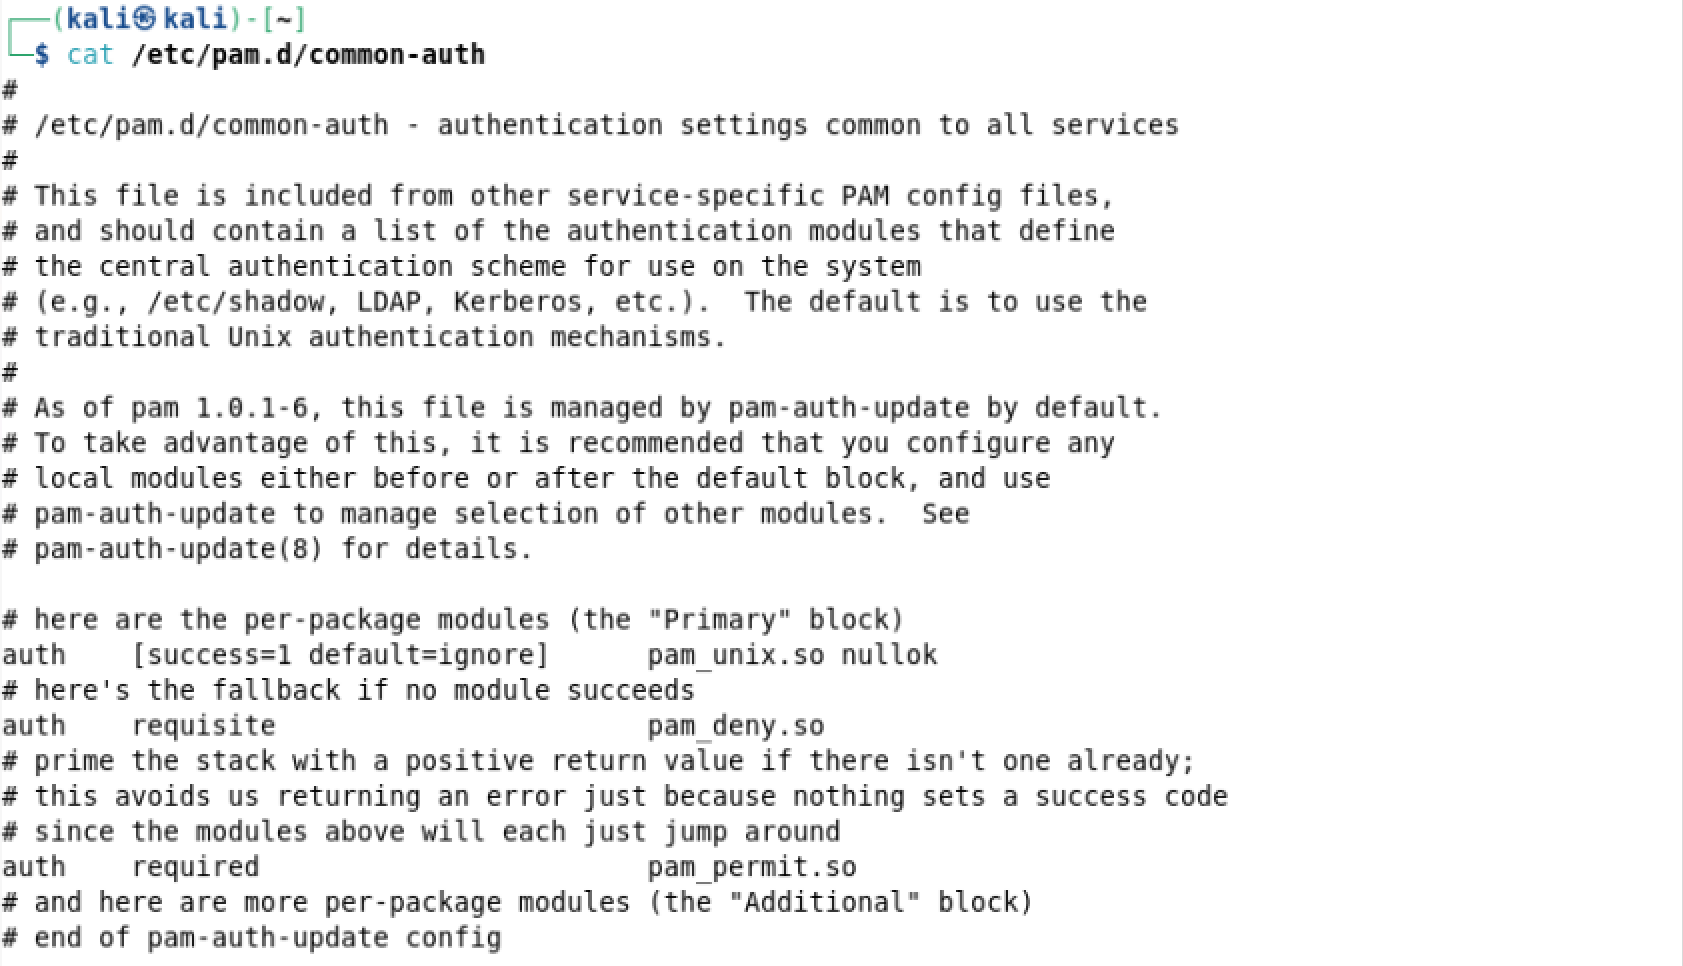
\includegraphics[width=0.50\textwidth]{images/p2.3.1.png}\\ \textit{Figure 17: Screenshot of current /etc/pam.d/common-auth file contents}\\
\ \\
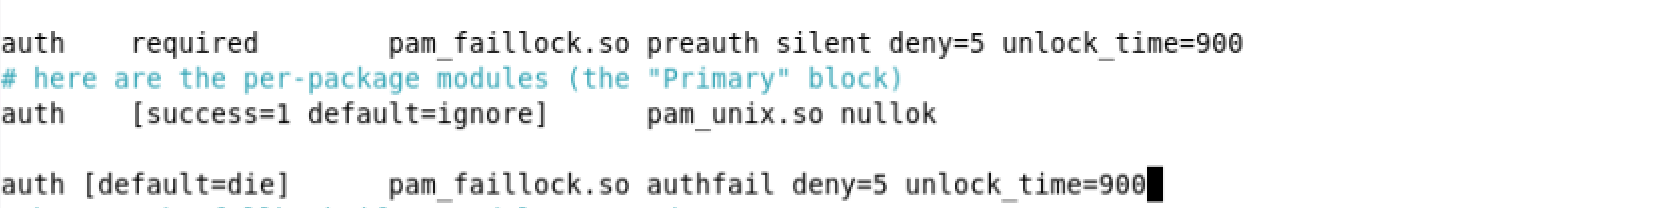
\includegraphics[width=0.50\textwidth]{images/p2.3.2.png}\\ \textit{Figure 18: Screenshot of two lines added to /etc/pam.d/common-auth file}\\
\ \\
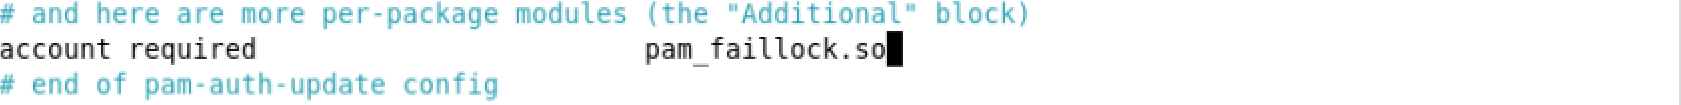
\includegraphics[width=0.50\textwidth]{images/p2.3.3.png}\\ \textit{Figure 19: Screenshot of line added to the end of /etc/pam.d/common-account file}\\
\ \\
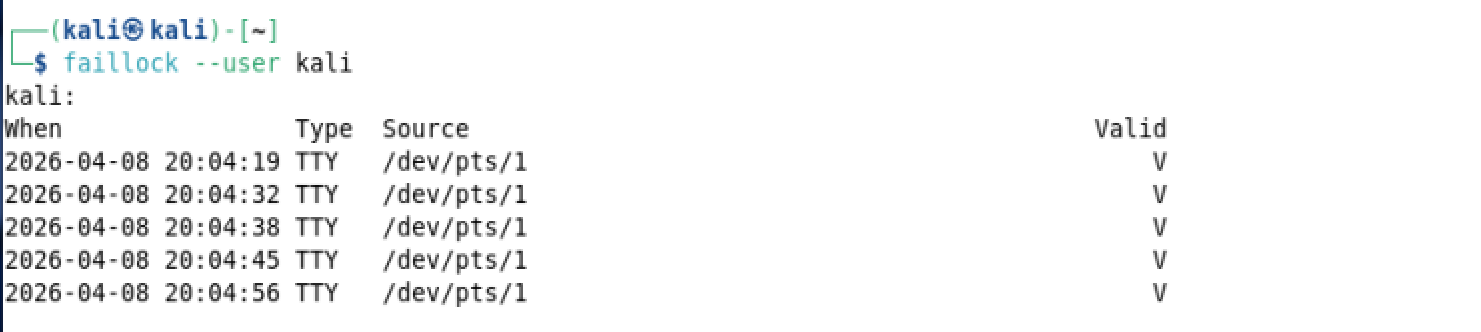
\includegraphics[width=0.50\textwidth]{images/p2.3.4.png}\\ \textit{Figure 20: Screenshot of faillock test results.}\\
\ \\
\underbar{Note about Section 2.3:} I had to do this section of the lab three times as there was an reoccurring issue with the password policy. For some reason, I kept getting locked out of my account immediately after implementing the password policy. After several tries, I asked for help, spun to before the lockout policy was implemented and continued with the rest of the lab.
% +++ P02.4 +++
\subsection{Review and Manage Services}
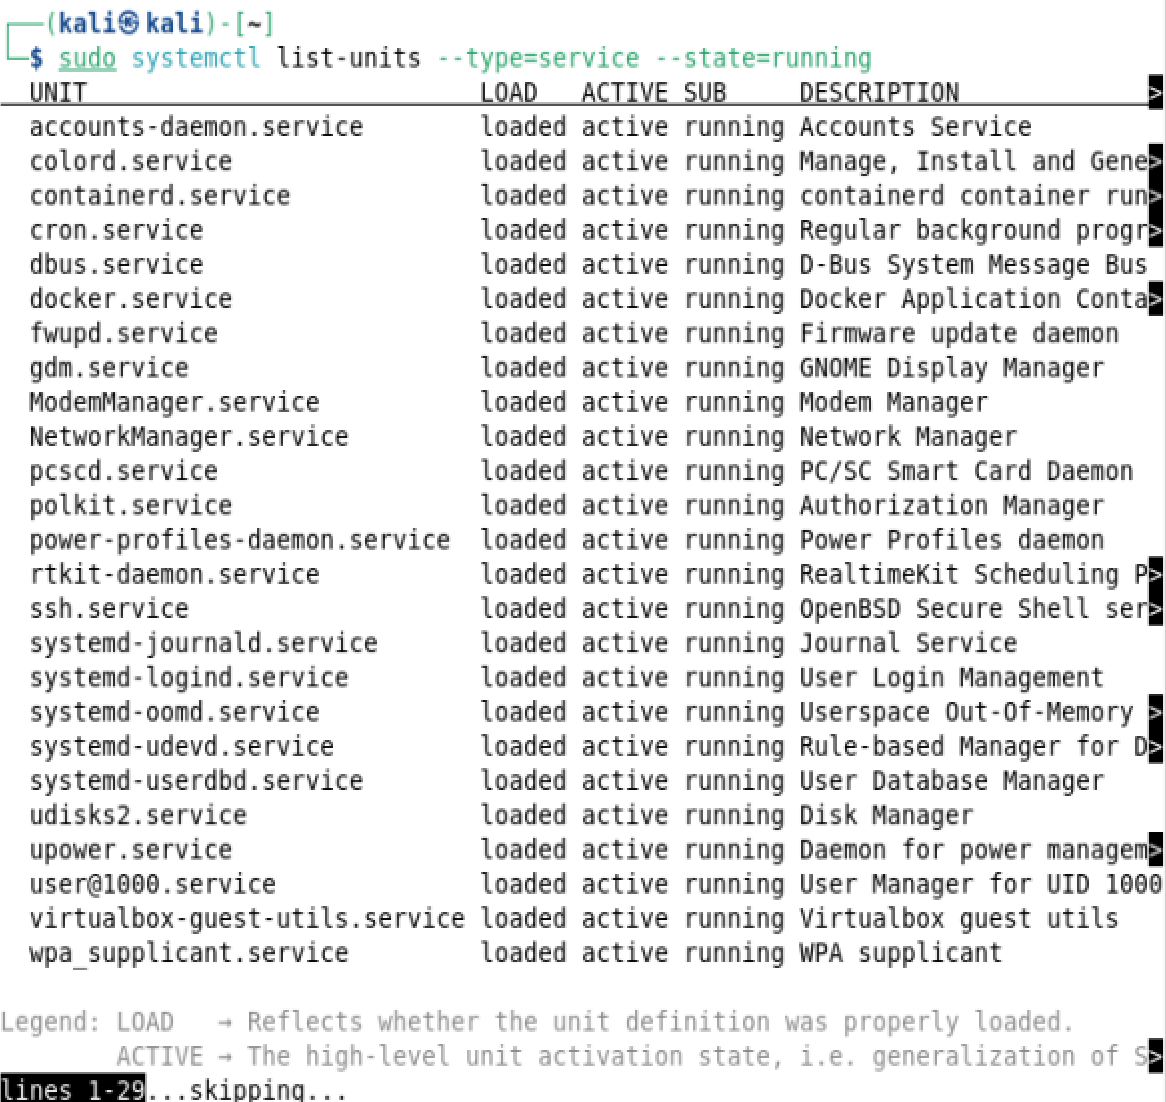
\includegraphics[width=0.50\textwidth]{images/p2.4.1.png}\\ \textit{Figure 21: Screenshot of running services}\\
\ \\
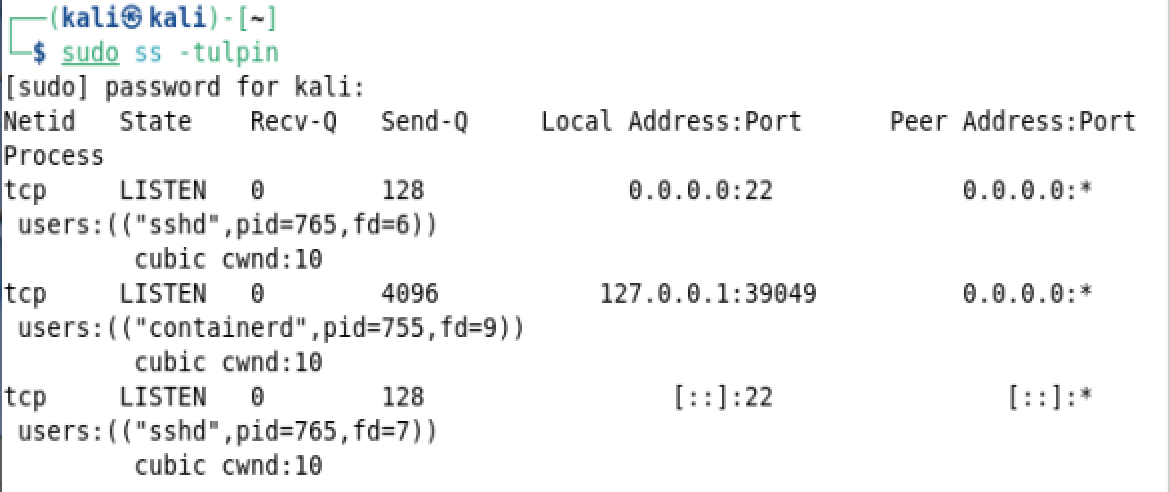
\includegraphics[width=0.50\textwidth]{images/p2.4.2.png}\\ \textit{Figure 22: Screenshot of listening ports}\\
\ \\
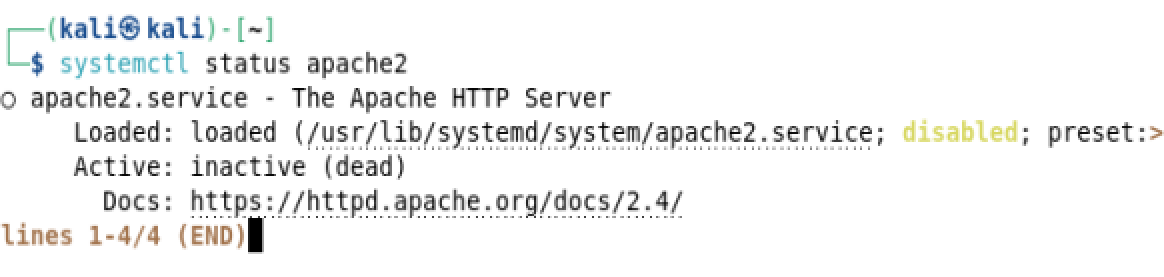
\includegraphics[width=0.50\textwidth]{images/p2.4.3.png}\\ \textit{Figure 23: Screenshot of apache2 disabled}\\
\ \\
\underbar{Note about this section:} I ran the check on all of the services listed in the Kali quick reference table and of all the services that were installed, only apache2 was active.
% +++ P02.5 +++
\subsection{SSH Hardening}
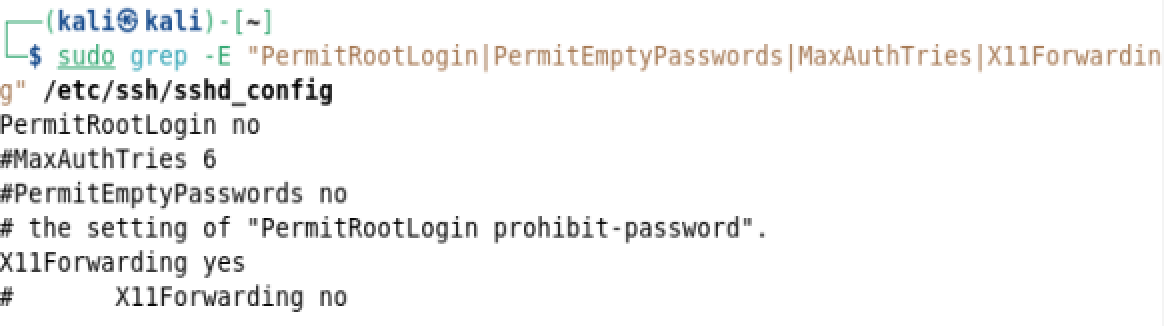
\includegraphics[width=0.50\textwidth]{images/p2.5.1.png}\\ \textit{Figure 24: Screenshot of current SSH daemon configuration}\\
\ \\
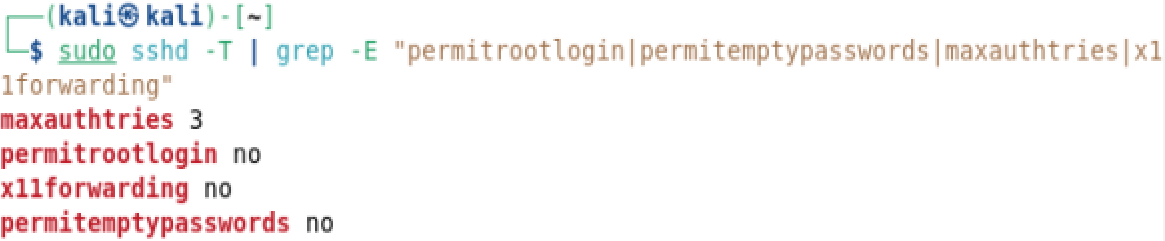
\includegraphics[width=0.50\textwidth]{images/p2.5.2.png}\\ \textit{Figure 25: Screenshot of hardened SSH configuration}\\

%=====================================================
% +++++ Part 03 +++++
\section{CIS Benchmark Comparison}
% +++ P03.1 +++
\subsection{Linux CIS Benchmark Checks}
\begin{enumerate}
	% +++ 1 +++
	\item \textbf{5.6.1.1} Ensure password expiration is 365 days or less
	\begin{itemize}
		\item \textbf{Check Command:}\texttt{grep PASS\underbar{   }MAX\underbar{   }DAYS /etc/login.defs}
		\item 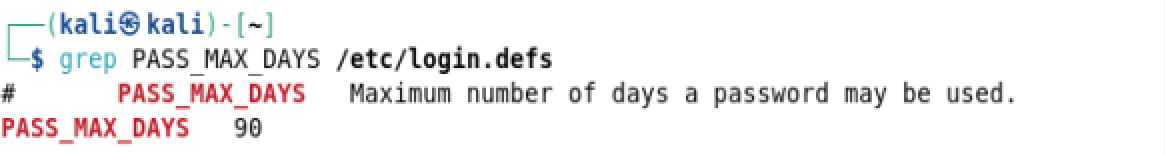
\includegraphics[width=0.60\textwidth]{images/p3.1.png} \\ \textit{Figure 26.1: Screenshot of check command output}
		\item \textbf{Result (Pass/Fail):} \texttt{PASS\underbar{   }MAX\underbar{   }DAYS   90} ; \textit{\textcolor{OliveGreen}{PASS}}
	\end{itemize}
	
	% +++ 2 +++
	\item \textbf{5.6.1.2} Ensure minimum days between password changes is 1 or more
	\begin{itemize}
		\item \textbf{Check Command:} \texttt{grep PASS\underbar{   }MIN\underbar{   }DAYS /etc/login.defs}
		\item 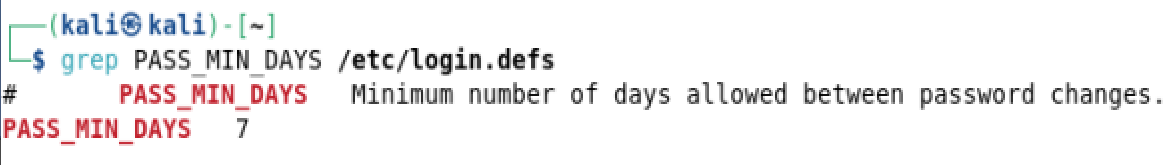
\includegraphics[width=0.60\textwidth]{images/p3.2.png} \\ \textit{Figure 26.2: Screenshot of check command output}
		\item \textbf{Result (Pass/Fail):} \texttt{PASS\underbar{   }MIN\underbar{   }DAYS   7} ; \textit{\textcolor{OliveGreen}{PASS}}
	\end{itemize}

	% +++ 3 +++
	\item \textbf{5.6.1.3} Ensure password expiration warning is 7 or more days
	\begin{itemize}
		\item \textbf{Check Command:} \texttt{grep PASS\underbar{   }WARN\underbar{   }AGE /etc/login.defs}
		\item 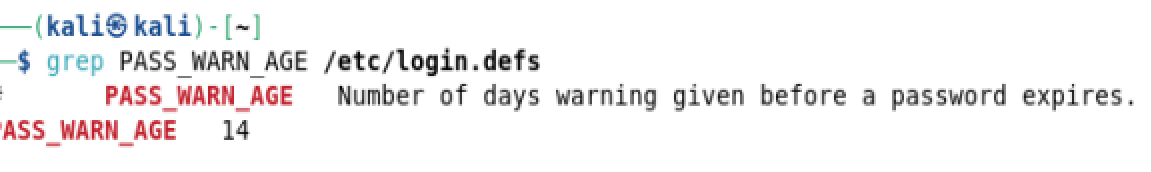
\includegraphics[width=0.60\textwidth]{images/p3.3.png} \\ \textit{Figure 26.3: Screenshot of check command output}
		\item \textbf{Result (Pass/Fail):} \texttt{PASS\underbar{   }WARN\underbar{   }AGE   14} ; \textit{\textcolor{OliveGreen}{PASS}}	
	\end{itemize}
	\newpage
	
	% +++ 4 +++
	\item \textbf{5.2.7} Ensure SSH root login is disabled
	\begin{itemize}
		\item \textbf{Check Command:} \texttt{sudo sshd -T | grep permitrootlogin}
		\item 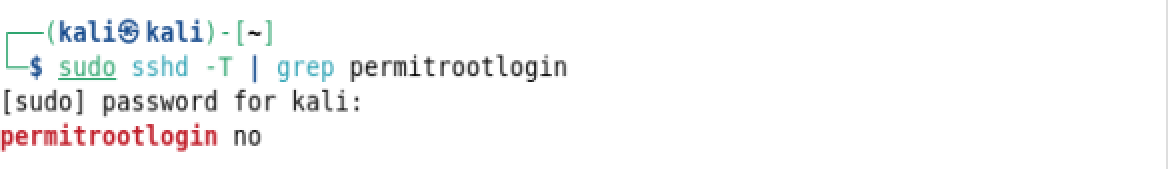
\includegraphics[width=0.60\textwidth]{images/p3.4.png} \\ \textit{Figure 26.4: Screenshot of check command output}
		\item \textbf{Result (Pass/Fail):} \texttt{permitrootlogin no} ; \textit{\textcolor{OliveGreen}{PASS}}
	\end{itemize}

	% +++ 5 +++
	\item \textbf{5.2.11} Ensure SSH MaxAuthTries is set to 4 or fewer
	\begin{itemize}
		\item \textbf{Check Command:} \texttt{sudo sshd -T | grep maxauthtries}
		\item 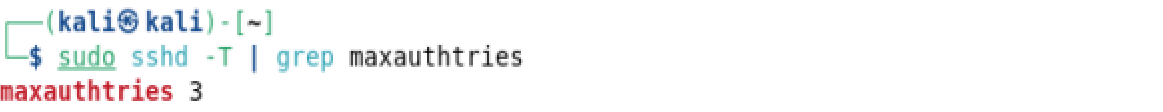
\includegraphics[width=0.60\textwidth]{images/p3.5.png} \\ \textit{Figure 26.5: Screenshot of check command output}
		\item \textbf{Result (Pass/Fail):} \texttt{maxauthtries 3} ; \textit{\textcolor{OliveGreen}{PASS}}
	\end{itemize}
\end{enumerate}

% +++ P03.2 +++
\subsection{Windows CIS Benchmark Checks}
\begin{enumerate}
	% +++ 1 +++
	\item \textbf{1.1.1} Ensure 'Enforce password history' is set to 5 or more passwords
	\begin{itemize}
		\item \textbf{Check Command:}
		\item \textit{Figure 26.6: Screenshot of...}
		\item \textbf{Result (Pass/Fail):}
	\end{itemize}

	% +++ 2 +++
	\item \textbf{1.1.4} Ensure 'Minimum password length' is set to 14 or more characters
	\begin{itemize}
		\item \textbf{Check Command:}
		\item \textit{Figure 26.7: Screenshot of...}
		\item \textbf{Result (Pass/Fail):}
	\end{itemize}

	% +++ 3 +++
	\item \textbf{1.2.1} Ensure 'Account lockout duration' is set to 15 or more minutes
	\begin{itemize}
		\item \textbf{Check Command:}
		\item \textit{Figure 26.8: Screenshot of...}
		\item \textbf{Result (Pass/Fail):}
	\end{itemize}
\end{enumerate}


% +++++ Part 04 +++++
\section{Security Policy Draft}

% +++++ Part 05 +++++
\section{Reflection Questions}
% +++ P05.1 +++
\subsection{Policy vs. Technical Controls}


% +++ P05.2 +++
\subsection{Defense in Depth}


\vfill
\textit{++report written with (minimal) help from Claude (Sonnet 4.6)++}
\end{document}

% +++++++++ Helpful stuff +++++++++++
%
% +++ Using Minipages +++
% \begin{minipage}[t]{\linewidth}
% \includegraphics[width=0.50\textwidth]{*Image file}\\
% \textit{*Image subtitle}
% \end{minipage}
% \end{enumerate}
%


% +++ Fixed width table +++
%\begin{tabularx}{1.0\textwidth}{
%	|| >{\raggedright\arraybackslash}X
%	|  >{\raggedright\arraybackslash}X
%	|  >{\raggedright\arraybackslash}X
%	|  >{\raggedright\arraybackslash}X || }
%	\hline
%	\textbf{x} & \textbf{x} & \textbf{x} & \textbf{x} \\
%	\hline \hline
%	x $ x $ x & x & x & x  \\
%	\hline
%	x $ x $ x & x & x & x \\
%	\hline
%	x $ x $ x & x & x & x \\
%	\hline
%	x $ x $ x & x &  x  & x \\
%	\hline
%\end{tabularx}
%

% +++ For tables that take multiple pages +++
%{\singlespacing
%	\begin{longtable}{
% 		|| >{\centering\arraybackslash}p{\colNum}
%  		| >{\raggedright\arraybackslash}p{\colSmall}
%  		| >{\raggedright\arraybackslash}p{\colSmall}
%  		| >{\raggedright\arraybackslash}p{\colBig}
%  		| >{\raggedright\arraybackslash}p{\colSmall} ||}
%		\hline
%		\textbf{x} & \textbf{x} & \textbf{x} & \textbf{x} & \textbf{x} \\
%		\hline\hline
%		\endhead
%		\hline
%  	    	 x & x & x & x  & x \\
%		\hline
%	\end{longtable}
%}












